\documentclass[11pt,a4paper]{article}
%%%%%%%%%%%%%%%%%%%%%%%%% Credit %%%%%%%%%%%%%%%%%%%%%%%%

% template ini dibuat oleh martin.manullang@if.itera.ac.id untuk dipergunakan oleh seluruh sivitas akademik itera.

%%%%%%%%%%%%%%%%%%%%%%%%% PACKAGE starts HERE %%%%%%%%%%%%%%%%%%%%%%%%
\usepackage{graphicx}
\usepackage{caption}
\captionsetup[table]{name=Tabel}
\captionsetup[figure]{name=Gambar}
\usepackage{tabulary}   
% \usepackage{amsmath}
\usepackage{fancyhdr}
% \usepackage{amssymb}
% \usepackage{amsthm}
\usepackage{placeins}
% \usepackage{amsfonts}
\usepackage{graphicx}
\usepackage[all]{xy}
\usepackage{tikz}
\usepackage{verbatim}
\usepackage[left=2cm,right=2cm,top=3cm,bottom=2.5cm]{geometry}
\usepackage{hyperref}
\hypersetup{
    colorlinks,
    linkcolor={red!50!black},
    citecolor={blue!50!black},
    urlcolor={blue!80!black}
}
\usepackage{libertine}
\usepackage{libertinust1math}
\usepackage[T1]{fontenc}
\usepackage{inconsolata}
\usepackage{float}

\usepackage{caption}
\usepackage{subcaption}
\usepackage{multirow}
\usepackage{psfrag}
\usepackage[T1]{fontenc}
\usepackage[scaled]{beramono}
% Enable inserting code into the document
\usepackage{listings}
\usepackage{xcolor} 
% custom color & style for listing
\definecolor{codegreen}{rgb}{0,0.6,0}
\definecolor{codegray}{rgb}{0.5,0.5,0.5}
\definecolor{codepurple}{rgb}{0.58,0,0.82}
\definecolor{backcolour}{rgb}{0.95,0.95,0.92}
\lstdefinestyle{mystyle}{
	backgroundcolor=\color{backcolour},   
	commentstyle=\color{green},
	keywordstyle=\color{codegreen},
	numberstyle=\tiny\color{codegray},
	stringstyle=\color{codepurple},
	basicstyle=\ttfamily\footnotesize,
	breakatwhitespace=false,         
	breaklines=true,                 
	captionpos=b,                    
	keepspaces=true,                 
	numbers=left,                    
	numbersep=5pt,                  
	showspaces=false,                
	showstringspaces=false,
	showtabs=false,                  
	tabsize=2
}
\lstset{style=mystyle}
\renewcommand{\lstlistingname}{Kode}
%%%%%%%%%%%%%%%%%%%%%%%%% PACKAGE ends HERE %%%%%%%%%%%%%%%%%%%%%%%%


%%%%%%%%%%%%%%%%%%%%%%%%% Data Diri %%%%%%%%%%%%%%%%%%%%%%%%
\newcommand{\stuid}{120140116}
\newcommand{\student}{\textbf{Muhammad Qomarudin (\stuid{})}}
\newcommand{\course}{\textbf{Sistem Operasi (IF2223)}}
\newcommand{\assignment}{\textbf{03}} % tugas ke...

%%%%%%%%%%%%%%%%%%% using theorem style %%%%%%%%%%%%%%%%%%%%
\newtheorem{thm}{Theorem}
\newtheorem{lem}[thm]{Lemma}
\newtheorem{defn}[thm]{Definition}
\newtheorem{exa}[thm]{Example}
\newtheorem{rem}[thm]{Remark}
\newtheorem{coro}[thm]{Corollary}
\newtheorem{quest}{Question}[section]
%%%%%%%%%%%%%%%%%%%%%%%%%%%%%%%%%%%%%%%%
\usepackage{lipsum}%% a garbage package you don't need except to create examples.
\usepackage{fancyhdr}
\usepackage[ddmmyyyy]{datetime}
\pagestyle{fancy}
\lhead{ \student }
\rhead{ \thepage}
\cfoot{\textbf{HandsOn 3 : Docker}} % ini untuk judul tugas
\renewcommand{\headrulewidth}{0.4pt}
\renewcommand{\footrulewidth}{0.4pt}

%%%%%%%%%%%%%%  Shortcut for usual set of numbers  %%%%%%%%%%%

\newcommand{\N}{\mathbb{N}}
\newcommand{\Z}{\mathbb{Z}}
\newcommand{\Q}{\mathbb{Q}}
\newcommand{\R}{\mathbb{R}}
\newcommand{\C}{\mathbb{C}}
\setlength\headheight{14pt}

%%%%%%%%%%%%%%%%%%%%%%%%%%%%%%%%%%%%%%%%%%%%%%%%%%%%%%%555

\begin{document}
\thispagestyle{empty}
\begin{center}
	
\includegraphics[scale = 0.15]{Figure/ifitera-header.png}
	\vspace{0.1cm}
\end{center}
\noindent
% change font family for header section only
%{\fontfamily{LinuxLibertineT-OsF}\large\selectfont 
{\large
\rule{17cm}{0.2cm}\\[0.3cm]
Nama: \student \hfill Tugas Ke: \assignment\\[0.1cm]
Mata Kuliah: \course \hfill Tanggal: \today\\
\rule{17cm}{0.05cm}
\vspace{0.1cm}
}


%%%%%%%%%%%%%%%%%%%%%%%%%%%%%%%%%%%%%%%%%%%%% BODY DOCUMENT %%%%%%%%%%%%%%%%%%%%%%%%%%%%%%%%%%%%%%%%%%%%%

\section{Tujuan HandsOn}
Tujuan dari HandsOn kali ini adalah untuk membuat mahasiswa memahami tentang Docker. Terutama
tentang perintah-perintah dasar yang digunakan dalam menggunakan Docker dan apa fungsi perintah tersebut, dan juga tentang 
istilah istilah yang sering di gunakan dalam penggunaan Docker.


\section{Instalisasi}
Pada HandsOn kali ini saya mengunakan Docker yang dijalankan pada sistem operasi Windows
\subsection{Requirements}
\subsubsection*{WSL 2 / Windows Subsytem for Linux}
WSL 2 atau Windows Subsytem for Linux adalah fitur yang di kembangkan oleh Microsoft yang menungkinkan 
sistem operasi Windows dapat menjalankan GNU/Linux untuk. untuk menginstall WSL 2, dapat kita lakukan melalui Windows PowerShell, dengan 
perintah berikut:
\begin{lstlisting}[language=bash]
	wsl --install #wsl default (ubuntu)

	wsl --install [disrto name] #install wsl untuk disrto khusus.
\end{lstlisting}
\begin{figure}[h]
\centering
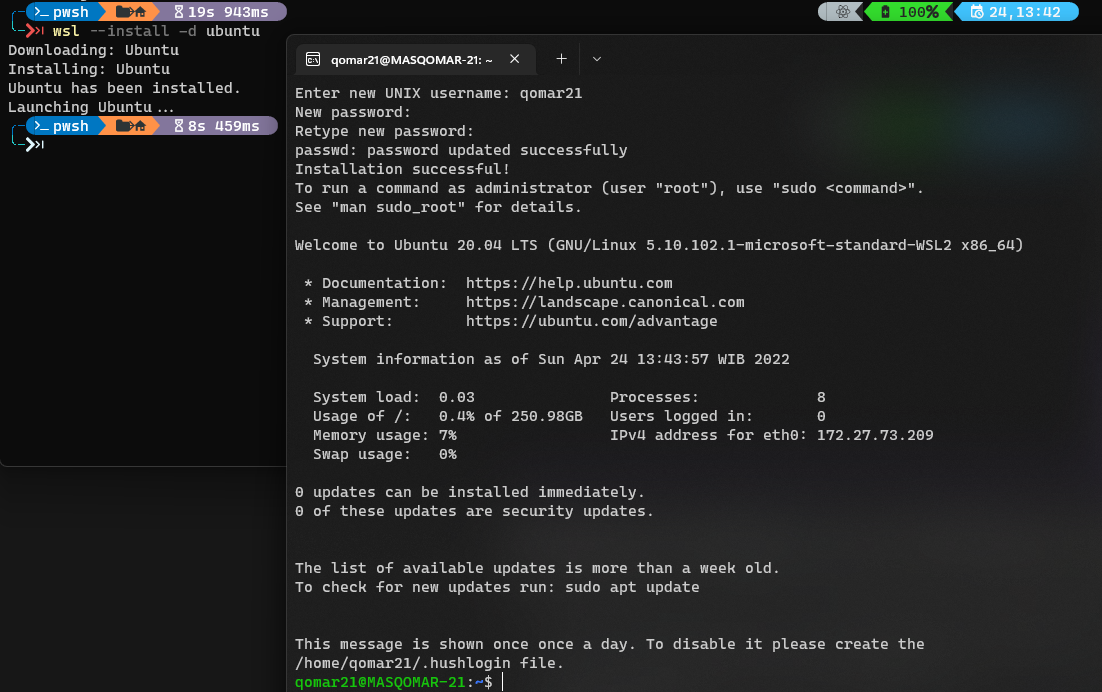
\includegraphics[width=0.7\textwidth]{Figure/asset/install wsl ubuntu.png}
\caption{Install WSL 2 melalui Windows PowerShell}
\end{figure}
selain mengunakan PowerShell, WSL juga dapat diinstall melalui Microsoft Store. dengan cara memasukan kata kunci "wsl" pada lolom Search. kemudian
meilih salah satu disrto yang akan di install, kemudail klik pada "get"
\begin{figure}[h]
\centering
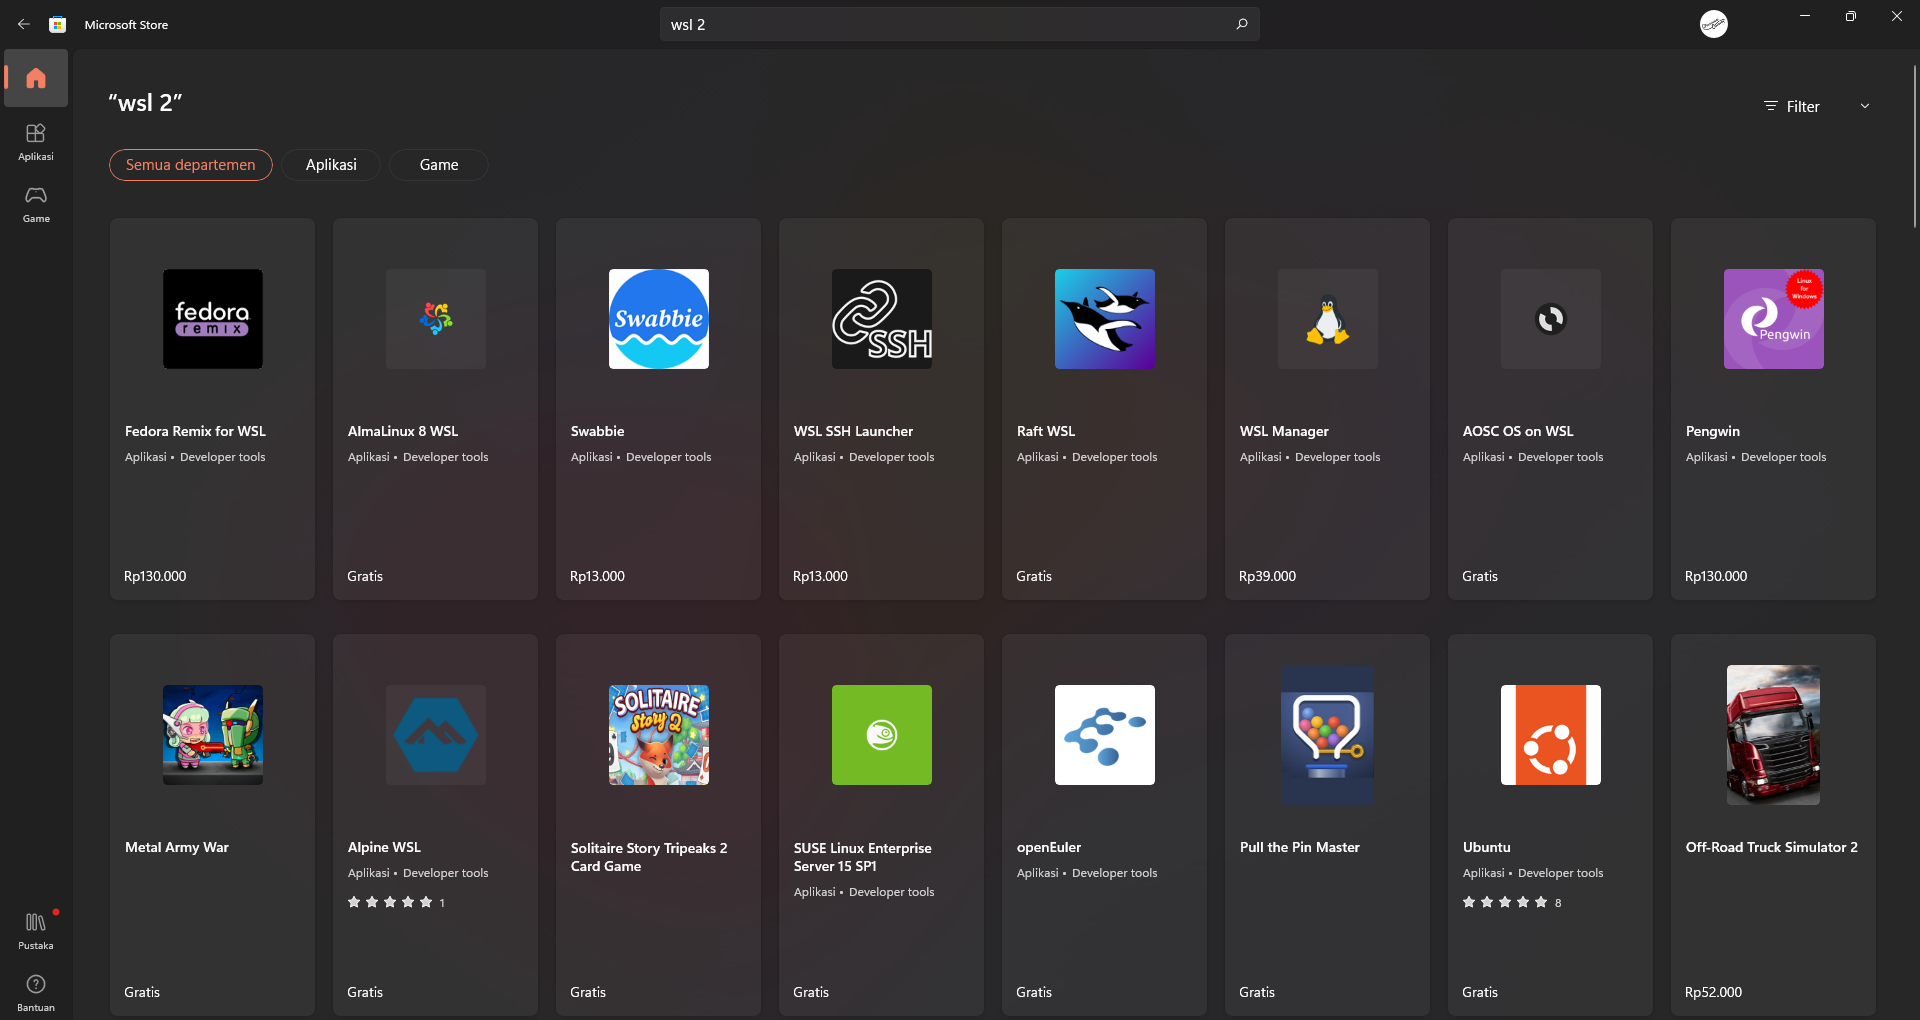
\includegraphics[width=0.7\textwidth]{Figure/asset/wsl from microsoft store.png}
\caption{Install WSL 2 melalui Microsoft Store}
\end{figure}

\subsection{install Docker}
Setelah WSL 2 diinstall, kita bisa menginstall Docker. Dengan cara kita mengunduh file installasi Docker melalui officila website resminya
\href{https://docs.docker.com/desktop/windows/install/}{Docker for Windows}. setelah selesai mengunduh, jalankan file
unduhan yang telah kita unduh tersebut. maka akan muncul Window seperti gambar di bawah ini, kemudain klik "Ok" maka mulai mengunduh
package-package yang diperlukan untuk menginstall Docker.
\begin{figure}[h]
\centering
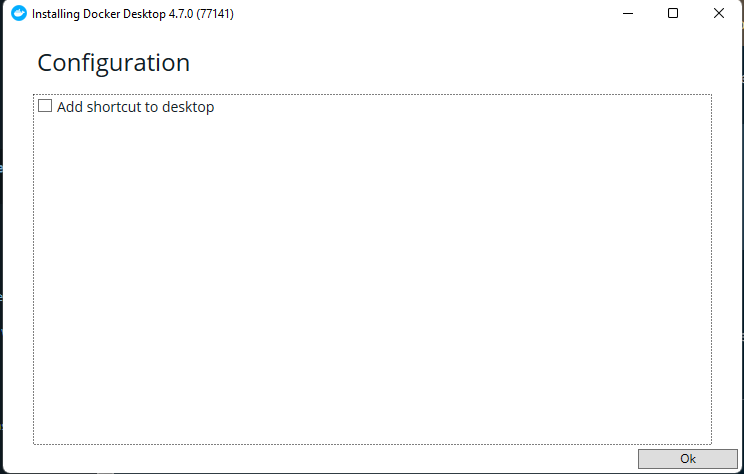
\includegraphics[width=0.7\textwidth]{Figure/asset/1.png}
\end{figure}

\begin{subfigure}[t]
\centering
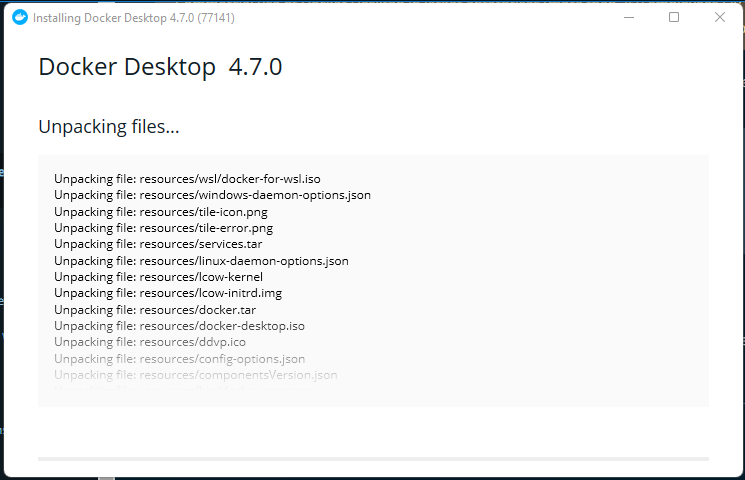
\includegraphics[width=0.7\textwidth]{Figure/asset/2.png}
\end{subfigure}

\begin{subfigure}[h]
	\centering
	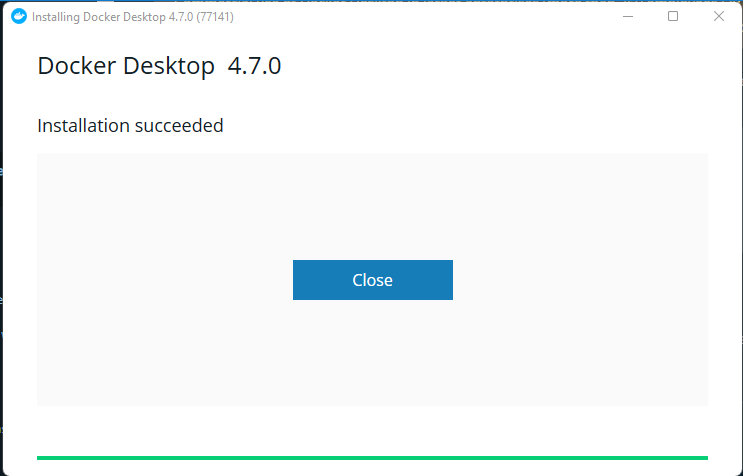
\includegraphics[width=0.7\textwidth]{Figure/asset/3.png}
\end{subfigure}



\end{document}